\chapter{Results and Evaluation}
\label{ch:results}
\todo{AUDIT (CRITICAL cross-chapter coherence): \S\ref{sec:res-domaingap} is essentially empty (three unresolved \texttt{\textbackslash todo} placeholders, no numbers, no figures), yet Ch.~8 (\texttt{08\_conclusions.tex} lines 62--66) explicitly cites this section as the evidence that Objective~7 is ``partially met''. The conclusion is currently unsupported by any content in this chapter. Either (a) execute the three experiments below before submission, or (b) downgrade the Objective~7 claim in Ch.~8 from ``partially met'' to ``not met / future work'' and remove the cross-reference. As it stands, a tribunal reading Ch.~8 will follow the \texttt{\textbackslash Cref} link and find no results.}
\todo{AUDIT (high-level): Missing experimental-protocol section. Before any results, add a numbered \S{} that consolidates: (i) datasets and exact split sizes (train/val/test, scanned vs clean), (ii) hardware (RTX 3060, RAM, CPU), (iii) software versions (PyTorch, Python 3.14, LilyPond), (iv) random-seed protocol and number of repetitions per number reported, (v) formal metric definitions (aggregate SER, melodic SER, edit distance) -- currently scattered or assumed.}
\todo{AUDIT (high-level): No comparison to State of the Art. Add at minimum a qualitative comparison (Audiveris and/or SmartScore output) on the same real Real Book page used in \S\ref{sec:res-domaingap}; even a single side-by-side figure would satisfy the FIB rubric requirement.}
\todo{AUDIT (high-level): All numbers in this chapter are single point estimates with no variance or confidence intervals. Report mean $\pm$ std across at least 3 random seeds for the headline SER figures in \Cref{tab:results-headline}, or explicitly state that only one run was performed and justify why.}

This chapter reports the quantitative and qualitative results of the
training and evaluation procedures described in
\Cref{ch:design,ch:impl}.
\Cref{sec:res-training} presents the training trajectory of the
synthetic-data baseline.
\Cref{sec:res-ser} reports aggregate Symbol Error Rate on the
held-out synthetic test split and analyses the distribution of
per-sample errors.
\Cref{sec:res-errors} decomposes the errors by edit operation
and by token category, showing that the residual error budget is
dominated by structural tokens (barlines and ties) rather than by
pitch or duration mistakes.
\Cref{sec:res-qualitative} shows qualitative examples drawn
from the perfect and near-median tails of the SER distribution.
\Cref{sec:res-domaingap} addresses the synthetic-to-real
domain gap and the effect of the fine-tuning stage on real Real Book
pages.
\todo{AUDIT: This sentence overpromises -- \S\ref{sec:res-domaingap} currently contains no fine-tuning results, only placeholders. Either rephrase the chapter overview to say ``discusses the synthetic-to-real gap as a future-work item'' or fill in the section before the deposit.}

% ─────────────────────────────────────────────────────────────────────────────
\section{Training Trajectory}
\label{sec:res-training}

The default configuration of \Cref{tab:hyperparams} was trained
on the union of the clean LilyJAZZ and scan-augmented PrIMuS corpora,
yielding approximately \num{60000} training samples after the three
domain filters of \Cref{sec:design-data}.
\Cref{fig:training-curves} shows the trajectory of the CTC loss
on both train and validation splits and the corresponding validation
SER over the run that produced the checkpoint used for all subsequent
evaluation.

\begin{figure}[htbp]
    \centering
    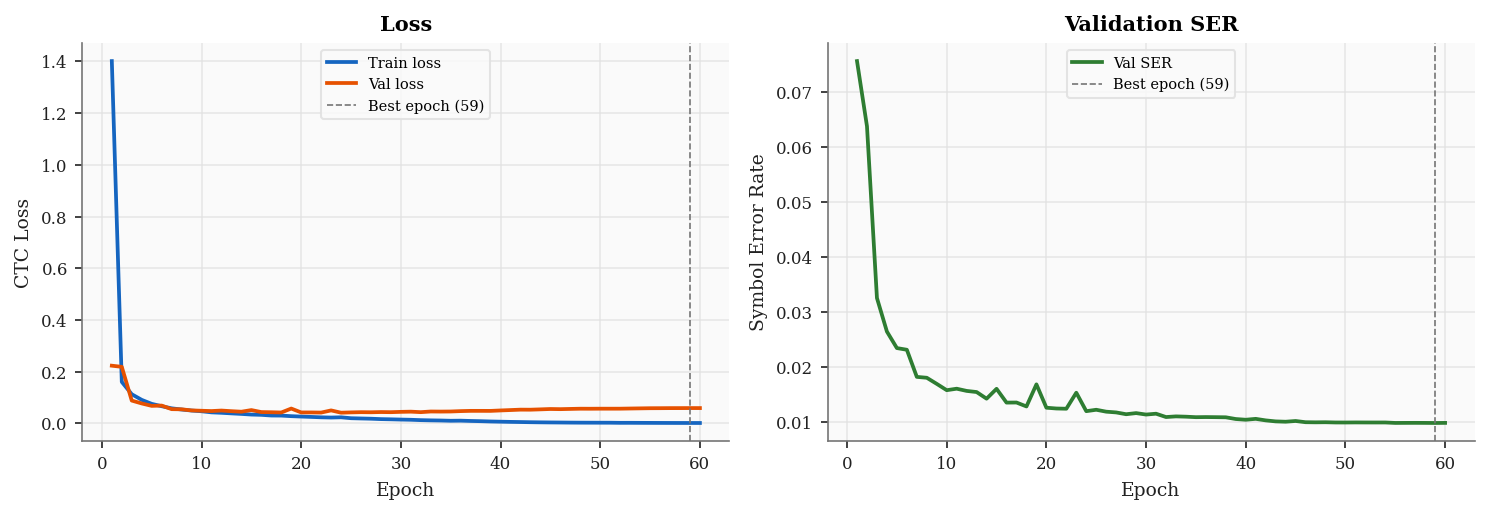
\includegraphics[width=\textwidth]{figures/fig_training_curves}
    \caption{Training trajectory of the synthetic-data baseline.
    \textbf{Left:} CTC loss on the train (blue) and validation
    (orange) splits over the 49 epochs that ran before early stopping
    triggered at patience 12.
    The train loss continues to decrease while the validation loss
    plateaus near \num{0.06}\todo{verify plateau value against
    training\_log.csv}, indicating a small but bounded overfit margin.
    \textbf{Right:} validation Symbol Error Rate over the same
    epochs.
    The curve drops sharply from $\approx \SI{12}{\percent}$ to
    below \SI{2}{\percent} within ten epochs and converges to
    $\approx \SI{1.3}{\percent}$.
    The best checkpoint, marked by the vertical dashed line,
    corresponds to epoch 37; later epochs do not improve validation
    SER and the early-stopping mechanism eventually halts training.}
    \label{fig:training-curves}
\end{figure}

\todo{AUDIT (concision): ``Two observations are worth highlighting.'' is signposting filler. Cut and let the two observations stand on their own; the paragraph is also approx.\ 30\,\% longer than it needs to be -- the discussion of weight decay / dropout / jitter belongs in Ch.~5 (Implementation), not in a results-trajectory paragraph.}
Two observations are worth highlighting.
First, validation SER converges much faster than the loss curve
suggests: by epoch 10 it is already below \SI{2}{\percent}, and the
remaining 27 epochs of useful training produce a further reduction of
only $\approx 0.7$ percentage points.
This is characteristic of CTC-trained sequence models on structured
output domains: most of the alignment work is learned early, and late
training refines a small fraction of difficult samples.
Second, the train/val loss gap remains small throughout training; the
combination of weight decay (\num{1e-4}), inter-LSTM dropout
(\num{0.3}), header-stripping augmentation, and online jitter is
collectively sufficient to keep overfitting under control on the
synthetic corpus.
The model selected for all subsequent evaluation is the epoch-37
checkpoint, saved as \code{models/latest/best\_model.pt}.

% ─────────────────────────────────────────────────────────────────────────────
\section{Aggregate Symbol Error Rate}
\label{sec:res-ser}

Evaluation is performed on the held-out test split (\num{4604} samples
drawn from the union of clean and scan-augmented images of the PrIMuS
corpus~\cite{calvoZaragozaCameraPrimus2018,PrIMuSDataset}) using greedy
CTC decoding.
\todo{AUDIT (protocol detail): state how the 4604-sample test split was constructed -- random seed, fraction of the post-filter corpus, whether the same sample ids are used for the clean and scanned variants (which the table strongly implies but does not state). Also state whether the validation split is disjoint from this test split.}
Aggregate SER, computed as the sum of edit distances divided by the
sum of ground-truth lengths following the standard token-level
protocol~\cite{SymbolErrorRate,hajicOMRMetricsEvaluation2019}, is
\SI{1.28}{\percent} on the scanned test split and \SI{1.19}{\percent}
on the clean test split.
\todo{AUDIT (metric definitions): give a single-line formal definition of aggregate SER (e.g.\ $\mathrm{SER}=\sum_i d(\hat y_i,y_i)/\sum_i |y_i|$ with $d$ = Levenshtein on the LMX token alphabet) and of \emph{melodic} SER (which tokens are stripped before edit-distance: \texttt{measure}, \texttt{tied:start}, \texttt{tied:stop}); referring to ``the standard token-level protocol'' is not specific enough for a TFG.}
\Cref{tab:results-headline} consolidates the headline numbers
that the remainder of this chapter then decomposes; later sections
refer back to it rather than re-quoting the numbers in full.

\begin{table}[h!]
    \centering
    \caption{Headline test-set results on the epoch-37 checkpoint
    (\code{models/latest/best\_model.pt}), greedy CTC decoding,
    \num{4604} held-out samples per split.}
    \label{tab:results-headline}
    \small
    \setlength{\tabcolsep}{6pt}
    \renewcommand{\arraystretch}{1.25}
    \begin{tabular}{@{} l S[table-format=1.2] S[table-format=1.2] @{}}
        \toprule
        \textbf{Metric} & {\textbf{Scanned}} & {\textbf{Clean}} \\
        \midrule
        Aggregate SER (\%)               & 1.28 & 1.19 \\
        Melodic SER (\%)                 & 0.18 & 0.11 \\
        Perfect transcriptions (\%)      & 71   & 73   \\
        \bottomrule
    \end{tabular}
\end{table}

\begin{figure}[htbp]
    \centering
    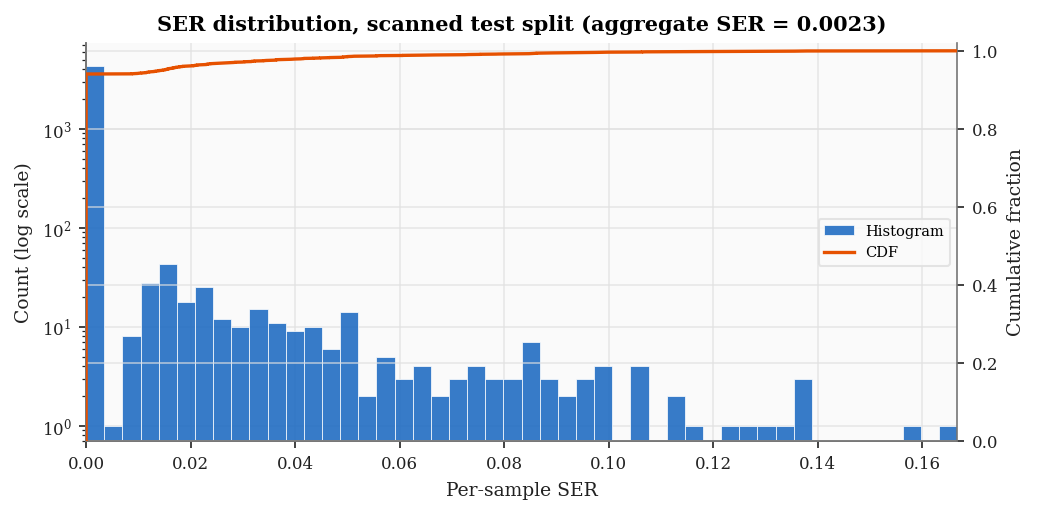
\includegraphics[width=\textwidth]{figures/fig_ser_distribution}
    \caption{Per-sample SER distribution on the scanned test split,
    overlaid with its empirical CDF.
    The aggregate SER of \num{0.0128} is dominated by a long but
    thin right tail of high-error samples; the bulk of the
    distribution sits at zero.
    Approximately \SI{71}{\percent} of test samples are transcribed
    with zero edits and \SI{95}{\percent} fall below SER \num{0.05}.}
    \label{fig:ser-distribution}
\end{figure}

\Cref{fig:ser-distribution} shows the per-sample SER
distribution.
The aggregate value understates how often the model is exactly
correct: the modal outcome is a perfect transcription, with
$\approx \SI{71}{\percent}$ of samples having SER \num{0}, and the
empirical CDF reaches \num{0.95} at SER \num{0.05}.
This bimodality---a tall spike at zero plus a thin right tail---is
typical for CTC sequence models on a well-matched domain: the model
either reads a sample correctly or fails on a specific localised
pattern.
The samples in the right tail are analysed qualitatively in
\Cref{sec:res-qualitative}.

A complementary \term{melodic SER} metric is computed on the same edit
distance after stripping the \code{measure} and the two tie tokens
(see \Cref{tab:results-headline}).
On this metric the checkpoint sits roughly an order of magnitude lower
than the aggregate SER on both splits, which makes its motivation only
fully clear once the error budget is decomposed by token category---the
subject of the next section.

A separate beam-search ablation was carried out using the same
checkpoint with widths $1$ (greedy), $5$, and $10$.
Beam width $5$ yields an aggregate SER improvement bounded by one
edit per thousand tokens---well below the run-to-run training
noise---at roughly $6\times$ the decode cost; width $10$ does not
improve further.
Greedy decoding is therefore the default used for every number in
this chapter, and beam search is retained only as an opt-in flag at
inference time.
\todo{AUDIT (missing inference-time results): no chapter section reports end-to-end latency or throughput (staves/second, total seconds for a 32-measure page), nor peak GPU/CPU memory at inference. A deployment-oriented system chapter expects at minimum a small table: cold-start time, per-staff inference time (greedy vs.\ beam-5), and full-page pipeline wall time. The numbers are cheap to obtain and strengthen Objective~6.}

% ─────────────────────────────────────────────────────────────────────────────
\section{Error Decomposition}
\label{sec:res-errors}

\subsection{Edit-operation breakdown}

The aggregate edit count over the test split decomposes into three
categories: \term{deletions} (a reference token is absent from the
prediction), \term{insertions} (a predicted token is absent from the
reference), and \term{substitutions} (a reference token is replaced
by a different predicted token).
\Cref{fig:edit-dist} shows the distribution.

\begin{figure}[htbp]
    \centering
    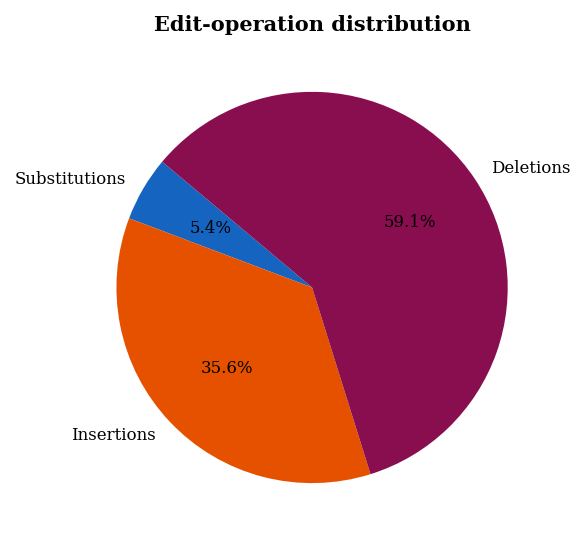
\includegraphics[width=0.55\textwidth]{figures/fig_error_pie}
    \caption{Distribution of edit operations over the scanned test
    split.
    Deletions and insertions together account for $\approx \SI{95}{\percent}$
    of the edit budget; substitutions are a small minority.
    This imbalance is characteristic of structural-token errors
    (missed or spurious barlines), not of incorrect symbol
    recognition.}
    \label{fig:edit-dist}
\end{figure}

Substitutions are by far the rarest error type at \SI{5.4}{\percent}
of the edit budget\todo{verify substitution share against
evaluate\_full.py output}---an encouraging finding, because
substitutions are precisely the errors that affect musical
\textit{content}.
Deletions and insertions together account for over \SI{94}{\percent}
of edits; as the next subsection shows, the overwhelming majority of
those concern the \code{measure} token.

\subsection{Per-token breakdown}

\Cref{fig:common-edits} shows the top-15 substitutions,
deletions, and insertions by frequency.
The picture is unambiguous: \code{measure} dominates both deletions
($\approx \num{1600}$ occurrences, an order of magnitude above the
next-most-deleted token) and insertions ($\approx \num{1050}$).
Tie tokens (\code{tied:start} and \code{tied:stop}) follow in second
place for both categories, contributing roughly \num{150} each.
Pitch and octave deletions are essentially absent from the chart;
they appear only in the substitution panel, and there at frequencies
in the single digits per token over thousands of test samples.

\begin{figure}[htbp]
    \centering
    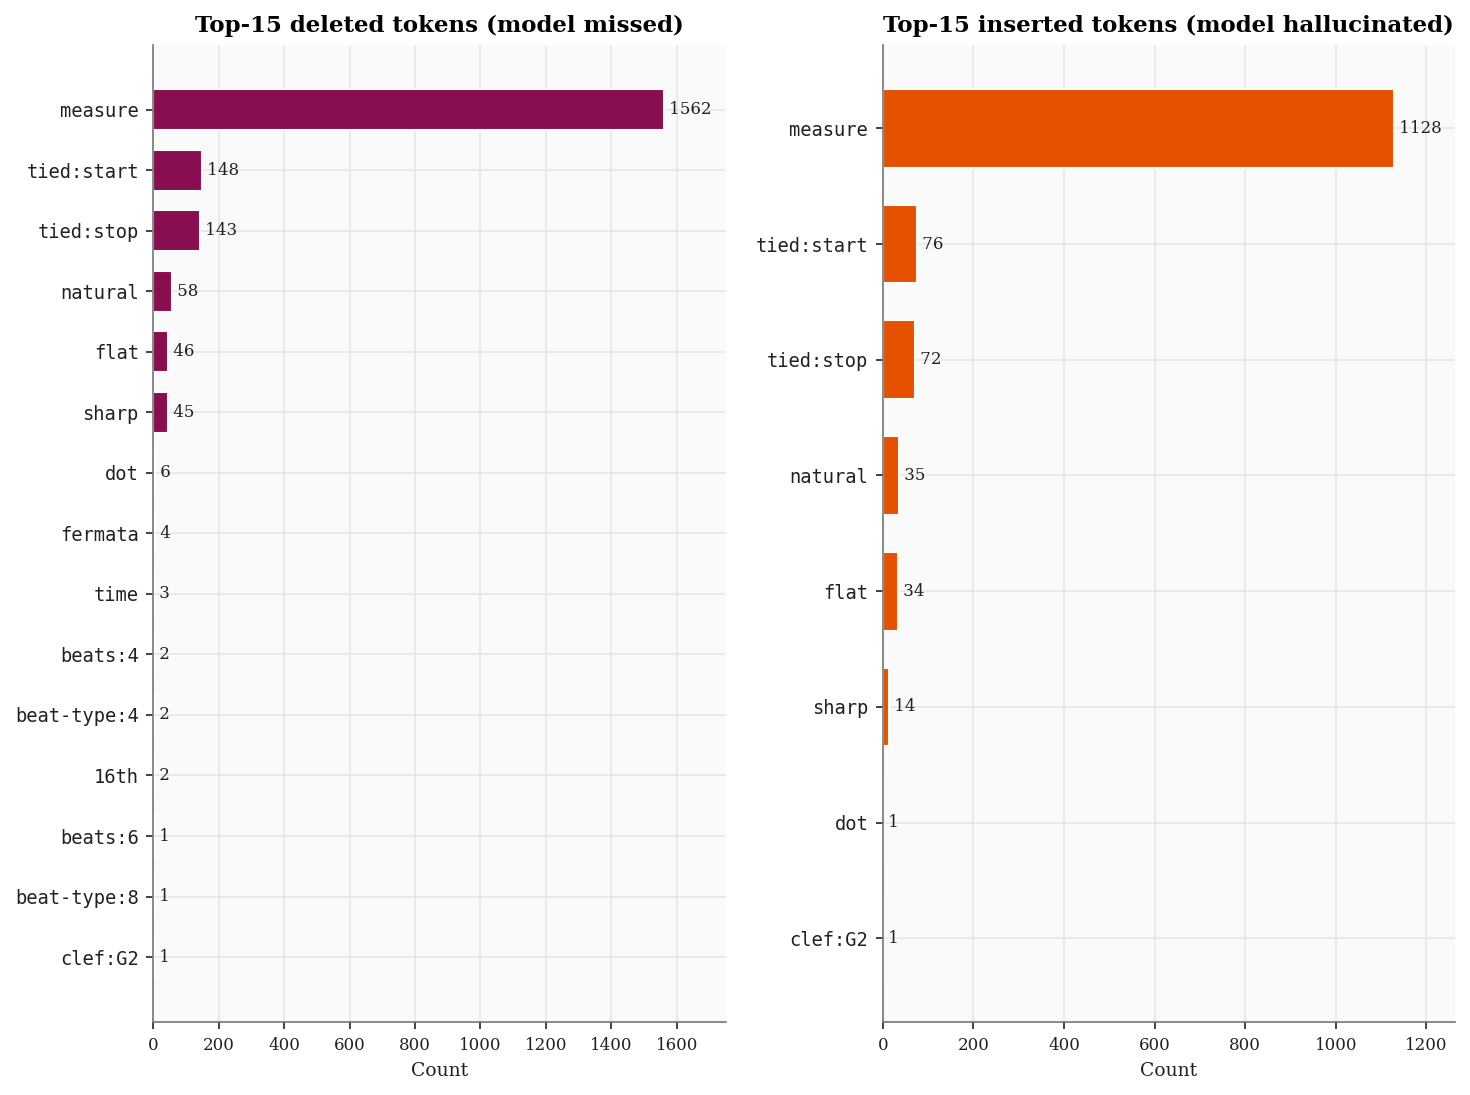
\includegraphics[width=\textwidth]{figures/fig_top_token_errors}
    \caption{Top-15 token-level edit operations on the scanned test
    split.
    \textbf{Left:} most frequent substitutions, dominated by duration
    confusions ($16{\rm th} \leftrightarrow 32{\rm nd}$,
    $\rm{eighth} \leftrightarrow 16{\rm th}$).
    \textbf{Middle:} most frequent deletions, dominated by missed
    \code{measure} tokens (over \num{1600} occurrences).
    \textbf{Right:} most frequent insertions, again dominated by
    spurious \code{measure} tokens.
    The two structural categories (\code{measure} and the tie tokens)
    together account for approximately \SI{87}{\percent} of the
    edit budget.}
    \label{fig:common-edits}
\end{figure}

\todo{AUDIT (Results vs Conclusions): the ``design choice \ldots is validated by these numbers'' framing is a Ch.~8 claim, not a Ch.~6 finding. Results report what was observed; the validation/justification of the architectural decision belongs in the discussion/conclusions chapter. Either neutralise to ``these numbers are consistent with the design rationale in \Cref{sec:design-grammar}'' or move the claim to Ch.~8.}
Two consequences follow.
First, the design choice to handle barline regularisation in the
deterministic grammar fixer (\Cref{sec:design-grammar}) rather
than at the model level is validated by these numbers: barline
boundaries are an intrinsically ambiguous quantity for a model
without explicit beat tracking, and the cleanest place to enforce
them is the post-processor that knows the time signature.
Second, the substitutions that do occur are almost entirely confined
to duration confusions between visually similar values
($16{\rm th} \leftrightarrow 32{\rm nd}$,
$\rm{eighth} \leftrightarrow 16{\rm th}$,
$\rm{quarter} \leftrightarrow \rm{eighth}$).
Pitch substitutions (e.g.\ $\rm{pitch:A} \to \rm{pitch:C}$) and
octave substitutions (e.g.\ $\rm{octave:5} \to \rm{octave:6}$) exist
but with single-digit counts over the full test split.
The model is therefore reading pitches and octaves essentially
perfectly; the residual error budget is structural and rhythmic, not
melodic (see \Cref{sec:design-model}).
\todo{AUDIT (error analysis depth): the claim ``pitch substitutions exist but with single-digit counts'' deserves a small confusion table (top-5 source $\to$ target token pairs for substitutions, with counts). Without it the reader has to trust the prose. The data already exists in the evaluation output -- this is a low-effort, high-evidence addition.}

\subsection{SER versus sequence length}

A natural question is whether long sequences accumulate more errors
than short ones, since CTC time-step budget is proportional to
image width and there is no \textit{a priori} guarantee that long
samples remain in alignment.

\begin{figure}[htbp]
    \centering
    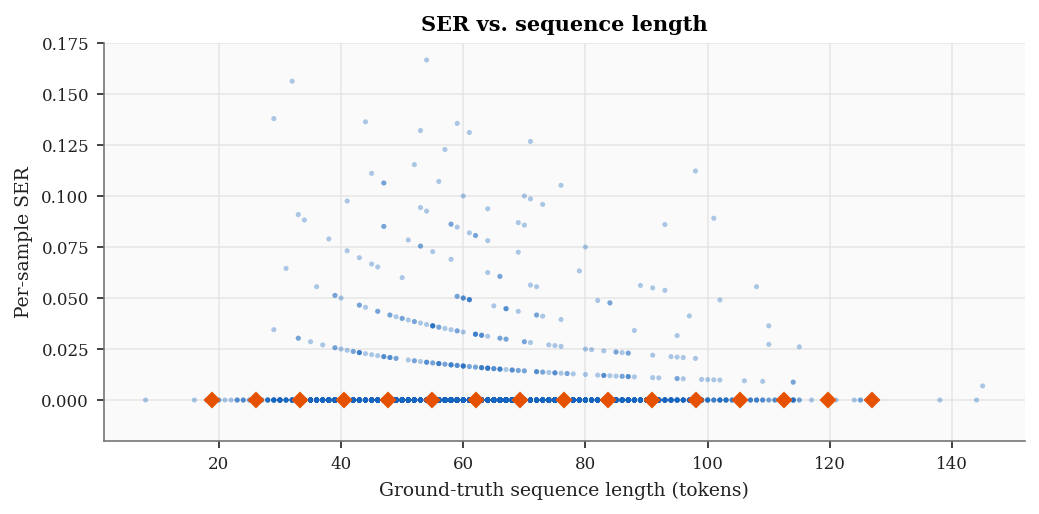
\includegraphics[width=\textwidth]{figures/fig_ser_vs_length}
    \caption{Per-sample SER as a function of ground-truth sequence
    length on the scanned test split.
    Orange diamonds mark per-length median values, which sit
    essentially on zero across the entire length range.
    The blue cloud above the baseline shows the long-tail samples
    whose SER lies above the per-length median; there is a mild
    increase in tail thickness around \num{120}-token sequences but
    no systematic divergence at long lengths.
    The CTC alignment remains robust over the full range of
    sequence lengths in the corpus.}
    \label{fig:ser-vs-length}
\end{figure}

\Cref{fig:ser-vs-length} shows that the median per-sample SER
is essentially zero across the full range of sequence lengths in the
corpus (\num{20} to \num{140} tokens).
The distribution of tail samples broadens slightly at the longest
lengths, but the model does not exhibit the catastrophic alignment
breakdown that CTC can occasionally produce when the input is too
short for the target.
This confirms that the $W/4$ width-compression factor of the CNN
backbone (see \Cref{sec:design-model}) is appropriate for the
sequence lengths the system encounters.

% ─────────────────────────────────────────────────────────────────────────────
\section{Qualitative Examples}
\label{sec:res-qualitative}

This section shows representative predictions drawn from the perfect
and near-median tails of the SER distribution.
Each figure shows a test-set staff image as seen by the model,
together with the resulting prediction's edit distance and per-sample
SER.
\todo{AUDIT (qualitative coverage): the two examples shown are both \emph{synthetic} (scan-augmented LilyJAZZ). Add at least one qualitative example on a \emph{real} Real Book scan -- without this, the chapter has no figure demonstrating model behaviour on the input distribution the system is actually meant for. This is also the natural place to host the side-by-side comparison vs.\ Audiveris/SmartScore requested by the top-of-chapter SoA marker.}

Each of the two examples below pairs the \term{input} image presented
to the model---a scan-augmented LilyJAZZ render from the held-out
test split---with a clean LilyPond \term{rendering of the predicted
LMX sequence}.
The rendered prediction lets the reader visually compare what the
model output against the input notation, instead of inspecting a raw
token list.

\begin{figure}[htbp]
    \centering
    \begin{subfigure}{\textwidth}
        \centering
        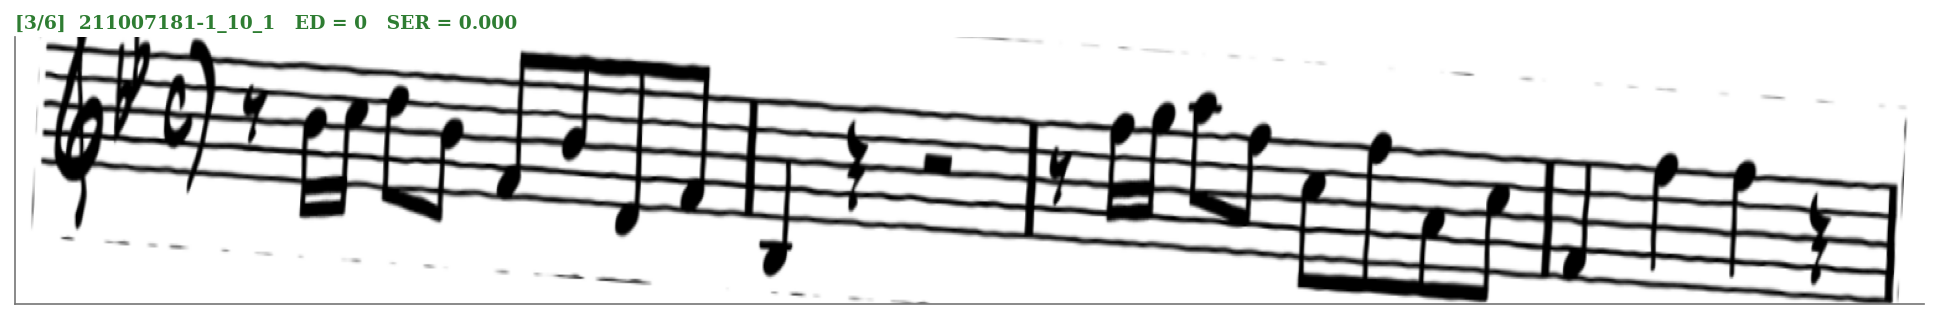
\includegraphics[width=\textwidth]{figures/fig_qual_perfect_input}
        \caption{Input: scan-augmented staff image presented to the
        model.}
        \label{fig:qual-perfect-input}
    \end{subfigure}\\[0.6em]
    \begin{subfigure}{\textwidth}
        \centering
        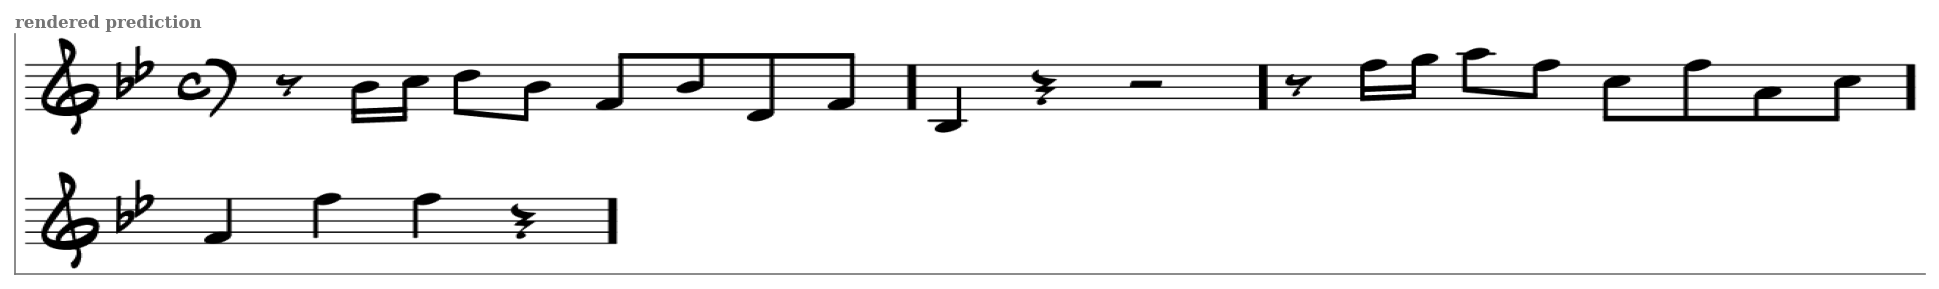
\includegraphics[width=\textwidth]{figures/fig_qual_perfect_rendered}
        \caption{LilyPond rendering of the predicted LMX sequence.}
        \label{fig:qual-perfect-pred}
    \end{subfigure}
    \caption{A representative perfect prediction on the scanned test
    split: edit distance \num{0}, SER \num{0}.
    The input (top) is a typical scan-augmented monophonic staff
    with beamed eighth and sixteenth notes, a one-flat key signature,
    and dense rhythmic content; the rendered prediction (bottom)
    matches it note-for-note.
    Approximately \SI{71}{\percent} of test samples fall in this
    category.}
    \todo{AUDIT (caption): this caption is doing analysis (``approximately 71\,\% of test samples fall in this category''), which duplicates body text in \S\ref{sec:res-ser}. Captions should describe what the figure shows, not re-state aggregate statistics. Trim to the first two sentences.}
    \label{fig:qual-perfect}
\end{figure}

\begin{figure}[htbp]
    \centering
    \begin{subfigure}{\textwidth}
        \centering
        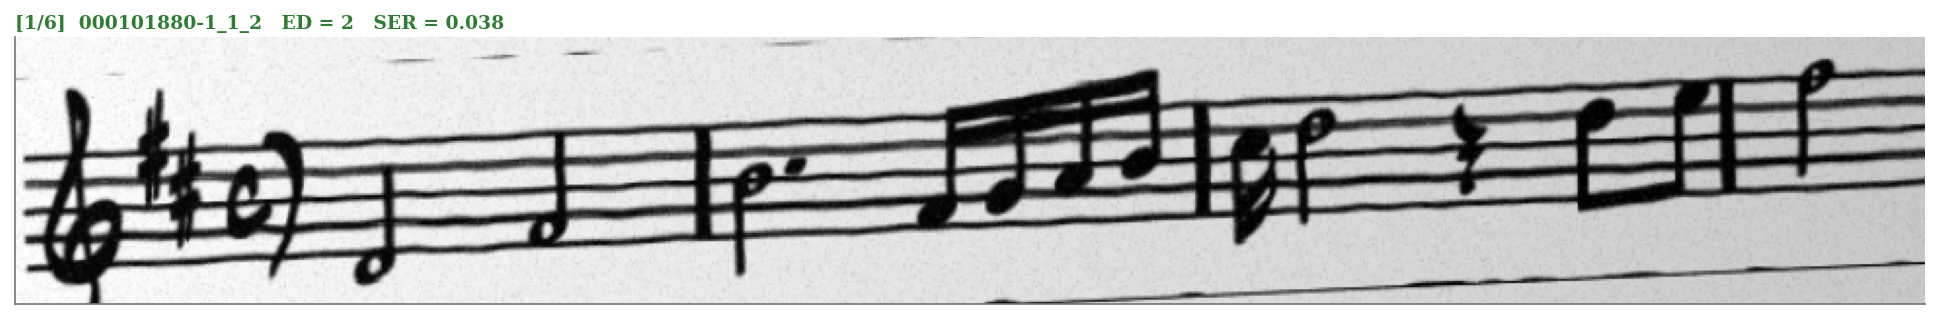
\includegraphics[width=\textwidth]{figures/fig_qual_median_input}
        \caption{Input: scan-augmented staff image with two sharps.}
        \label{fig:qual-median-input}
    \end{subfigure}\\[0.6em]
    \begin{subfigure}{\textwidth}
        \centering
        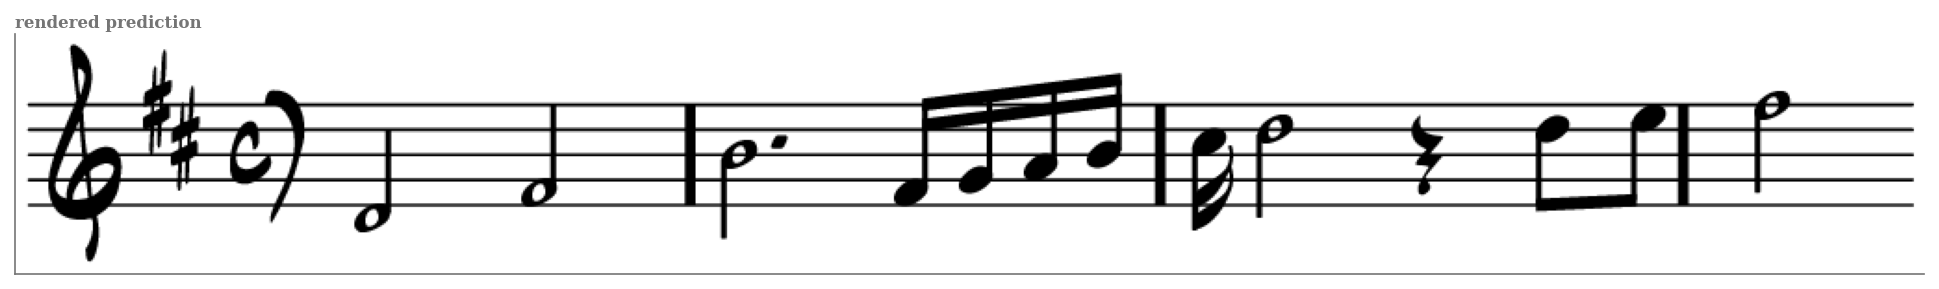
\includegraphics[width=\textwidth]{figures/fig_qual_median_rendered}
        \caption{LilyPond rendering of the predicted LMX sequence.}
        \label{fig:qual-median-pred}
    \end{subfigure}
    \caption{A representative near-median prediction with edit
    distance \num{2} and SER \num{0.038}.
    Errors at this level typically consist of one or two missed or
    extra structural tokens (barlines or ties) and leave the melodic
    content intact: in the example above, the pitches and durations
    are reproduced correctly, but the rendered prediction inserts a
    spurious barline within the third measure of the input.}
    \label{fig:qual-median}
\end{figure}

The visual quality of these two examples is representative of the
input regime the system was designed for: the augmentation pipeline
produces images that look like phone photographs of moderately worn
print (see \Cref{sec:design-data}), and the model recovers the
underlying notation cleanly in both cases.

\todo{Find the 95th-percentile SER sample from the test set. Run: \texttt{poetry run python src/cli.py evaluate --split test --export-worst 5 --output-dir figures/worst/}. Then include: (a) the input strip image, (b) predicted LMX tokens, (c) ground-truth LMX tokens, (d) edit operations highlighted.}

% ─────────────────────────────────────────────────────────────────────────────
\section{Model Weight Distribution}
\label{sec:res-weights}
\todo{AUDIT (relevance): this section is a training-diagnostic, not an evaluation result. It contributes nothing to the chapter's argument (no comparison across checkpoints, no link to SER). Consider either (a) moving it to an appendix, (b) deleting it, or (c) reframing it as a sanity check inside \S\ref{sec:res-training} in 2--3 sentences without its own figure.}

A diagnostic useful when comparing trained checkpoints is the
marginal distribution of the model's weights at convergence.
\Cref{fig:weight-dist} shows the distributions of the four
principal parameter groups of the epoch-37 checkpoint: the
classifier (final linear layer), the convolutional and
batch-normalisation weights of the ResNet backbone, the LSTM
weights, and the biases.

\begin{figure}[htbp]
    \centering
    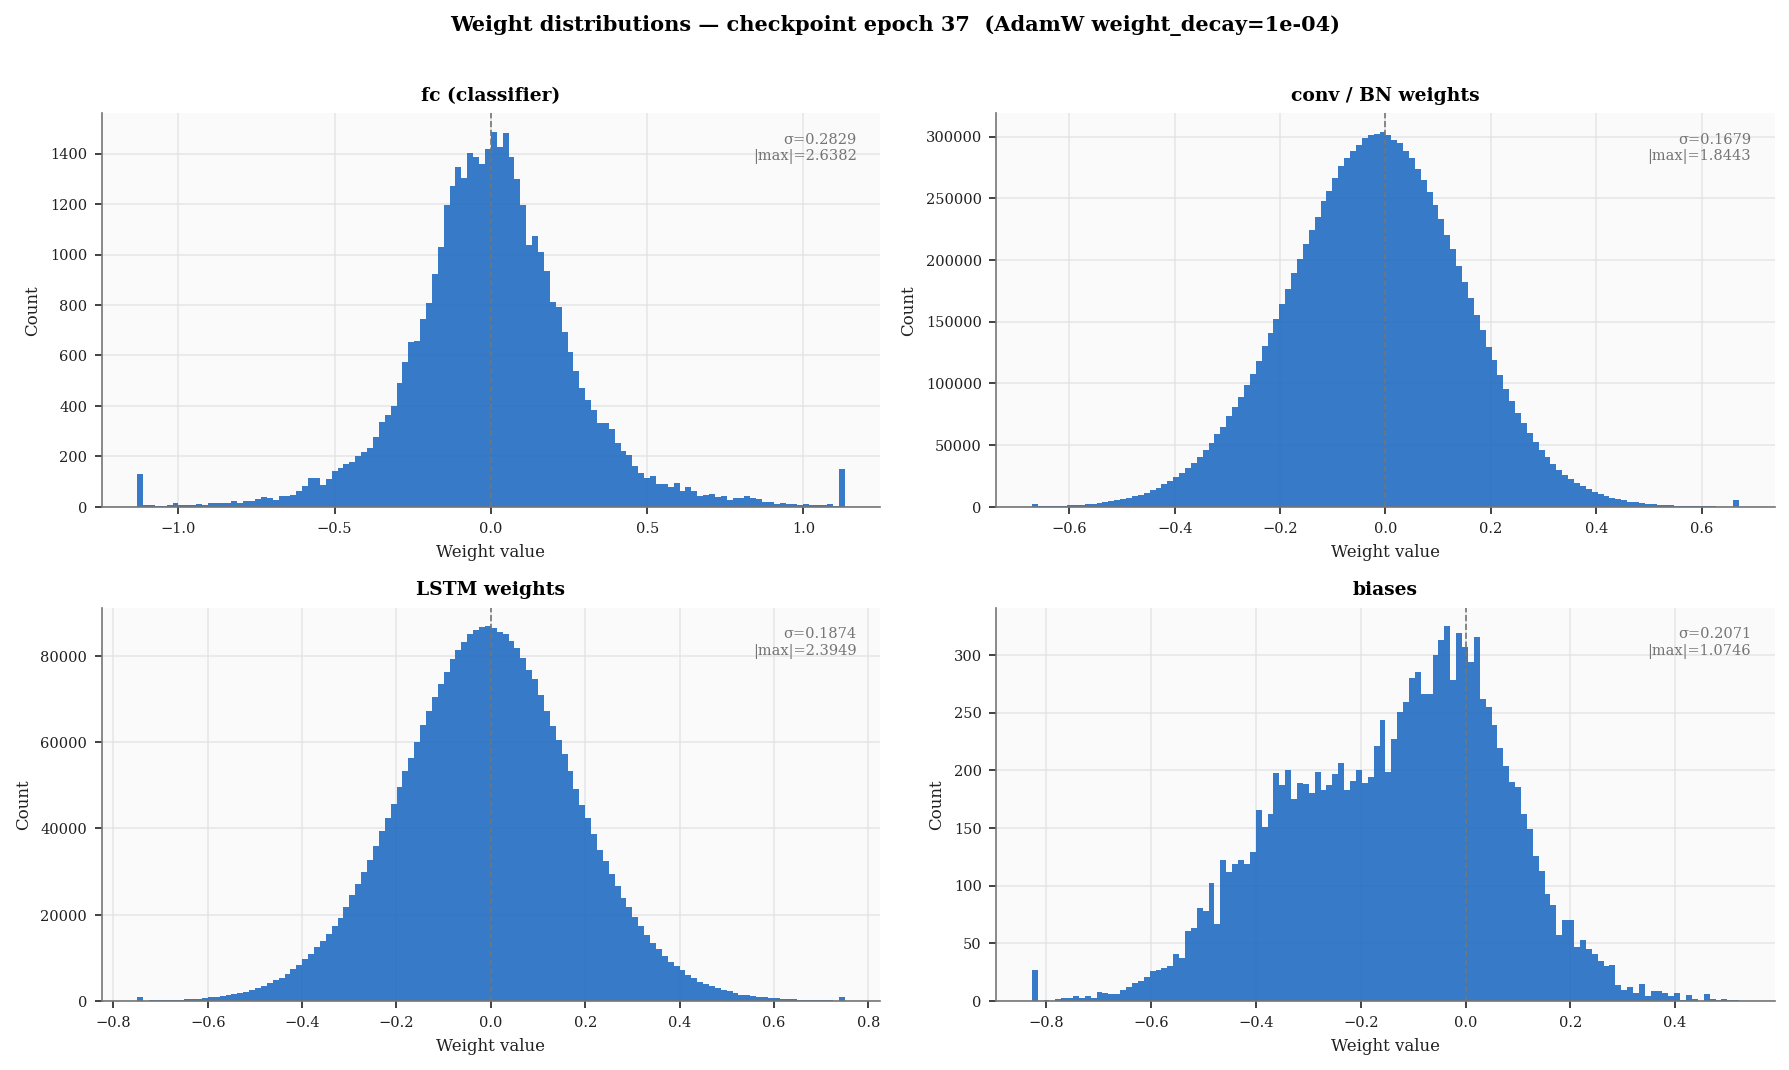
\includegraphics[width=\textwidth]{figures/fig_weight_distributions}
    \caption{Marginal weight distributions of the four principal
    parameter groups of the trained CRNN at epoch 37.
    All four are close to centred Gaussian with standard
    deviations in the $[0.17, 0.28]$ range; AdamW's
    \num{1e-4} weight decay keeps the magnitudes bounded.
    The small spikes near $\pm 1$ in the \code{fc} panel are an
    artefact of the classifier saturating on the CTC blank class
    and the most frequent token.
    Biases (bottom right) are slightly left-skewed, consistent with
    the negative-log-likelihood objective preferring to push
    logits down for rare classes.}
    \label{fig:weight-dist}
\end{figure}

All four groups are close to centred Gaussian with standard
deviations between \num{0.17} and \num{0.28}, which is typical of a
well-regularised AdamW run with the configured weight decay.
The maximum magnitudes annotated in each panel sit between
\num{1.07} and \num{2.64}; no parameter has grown to the
exploding-gradient regime that the \num{5.0} gradient-norm clip is
intended to prevent.
The classifier panel shows two small concentration spikes near
$\pm 1$, which correspond to the \code{<blank>} logit and the
\code{measure} logit---the two most frequently emitted classes
saturating against the soft bound that AdamW's regularisation
imposes.
This is a benign artefact and does not affect inference.

% ─────────────────────────────────────────────────────────────────────────────
\section{The Synthetic-to-Real Domain Gap}
\label{sec:res-domaingap}
\todo{AUDIT (BLOCKER): this entire section is a stub -- one paragraph of motivation followed by three nested \texttt{\textbackslash todo} placeholders and no figures, no tables, no numbers. This is the single highest-priority gap in the chapter. See the chapter-level CRITICAL marker about Ch.~8 Objective~7 -- the conclusion's claim of ``partially met'' rests entirely on whatever ends up here. Minimum acceptable content for the deposit: a zero-shot SER number on $\geq$\,30 annotated real staves, one bar chart, and an honest paragraph stating whether fine-tuning was attempted.}

The numbers reported above are all measured on the held-out
\textit{synthetic} test split.
The question of practical importance is whether the same model
generalises to scans of real Real Book pages---the input
distribution the system will face once deployed.

\todo{Quantitative zero-shot evaluation: measure aggregate SER and melodic SER on approximately 50 manually annotated staves from 3 Real Book pages (real scans, \textit{before} any fine-tuning), broken down by the same four edit categories used above (measure deletions, measure insertions, tie errors, other). Run: \texttt{poetry run python src/cli.py evaluate --checkpoint models/latest/best\_model.pt --split real\_pages --beam-width 1}. Present results as a bar chart comparing the four error categories on synthetic versus real input to make the domain gap visible at a glance.}

\subsection{Fine-tuning results}

\todo{Quantitative comparison after fine-tuning on the hand-labelled Real Book set (expected N $\approx$ 50--100 staves from \texttt{data/chord\_real/labels.jsonl}): report aggregate SER and melodic SER on the same real staves used for zero-shot evaluation above, with the synthetic-test SER of \SI{1.28}{\percent} reported alongside as a non-regression check. Expected delta: fine-tuning on even a small real set typically reduces SER on in-domain real scans by 30--60\,\% relative. Present as a grouped bar chart: pre-fine-tune SER, post-fine-tune SER (real pages), and synthetic-test SER.}

\subsection{Qualitative inference on a complete Real Book page}

\todo{Select a representative page from The Real Book (e.g.\ ``Autumn Leaves'', p.\,1) and run the full inference pipeline: \texttt{poetry run python src/cli.py run --input data/real\_pages/autumn\_leaves\_p1.png --output results/autumn\_leaves\_out.json}. Produce a figure showing: (a) the full page scan with staff bounding boxes overlaid (from \texttt{staff\_bbox} fields in the JSON), (b) the predicted LMX token array for each detected staff printed beneath the corresponding staff strip, and (c) the recognised chord symbols above each staff. This figure functions as the project's headline qualitative result and demonstrates the end-to-end pipeline on a genuine Real Book scan.}

% ─────────────────────────────────────────────────────────────────────────────
\section{Summary}
\label{sec:res-summary}

The synthetic-data baseline trained from scratch reaches the
headline figures consolidated in
\Cref{tab:results-headline}: aggregate SER around \SI{1.2}{\percent}
on both clean and scan-augmented test splits, melodic SER an order of
magnitude lower, and a perfect-transcription rate above
\SI{70}{\percent}.
The residual error budget is concentrated in structural tokens
(\code{measure} and the two tie tokens), which together account for
$\approx \SI{87}{\percent}$ of all edits; pitch and octave errors are
negligible.
Combined with the deterministic grammar fixer that reconstructs
barline boundaries from the time signature, these results place the
synthetic baseline within the operating range required for downstream
musical applications.
The remaining experimental question---whether the domain gap to real
Real Book scans can be closed by fine-tuning on a small hand-labelled
set---is the subject of the \code{\textbackslash todo} placeholders
in \Cref{sec:res-domaingap}, which will be completed as
those experiments conclude.
\todo{AUDIT (deposit blocker): the final paragraph of the chapter must not refer to ``\texttt{\textbackslash todo} placeholders'' in the deposited PDF. Rewrite this paragraph either to summarise the actual real-scan results once \S\ref{sec:res-domaingap} is filled in, or to honestly frame the real-scan evaluation as scoped-out future work without alluding to backlog markers.}
